%!TEX root = thesis.tex

% datastore shape from http://www.texample.net/tikz/examples/data-flow-diagram/
\makeatletter
\pgfdeclareshape{datastore}{
  \inheritsavedanchors[from=rectangle]
  \inheritanchorborder[from=rectangle]
  \inheritanchor[from=rectangle]{center}
  \inheritanchor[from=rectangle]{base}
  \inheritanchor[from=rectangle]{north}
  \inheritanchor[from=rectangle]{north east}
  \inheritanchor[from=rectangle]{east}
  \inheritanchor[from=rectangle]{south east}
  \inheritanchor[from=rectangle]{south}
  \inheritanchor[from=rectangle]{south west}
  \inheritanchor[from=rectangle]{west}
  \inheritanchor[from=rectangle]{north west}
  \backgroundpath{
    %  store lower right in xa/ya and upper right in xb/yb
    \southwest \pgf@xa=\pgf@x \pgf@ya=\pgf@y
    \northeast \pgf@xb=\pgf@x \pgf@yb=\pgf@y
    \pgfpathmoveto{\pgfpoint{\pgf@xa}{\pgf@ya}}
    \pgfpathlineto{\pgfpoint{\pgf@xb}{\pgf@ya}}
    \pgfpathmoveto{\pgfpoint{\pgf@xa}{\pgf@yb}}
    \pgfpathlineto{\pgfpoint{\pgf@xb}{\pgf@yb}}
 }
}
\makeatother

\tikzstyle{box}=[draw, thick, text centered, text width=2.5cm, node distance=1.5cm and 3cm, inner sep=.2cm]
\tikzstyle{datastore}=[box, shape=datastore]
\tikzstyle{process}=[box, rectangle]
\tikzstyle{terminator}=[box, rounded corners]
\tikzstyle{class}=[box, rectangle split, rectangle split parts=2]
\tikzstyle{line}=[->,>=stealth',shorten >=1pt, semithick, font=\footnotesize]
\tikzstyle{container}=[text width=3cm]

\chapter{Anwendung: Twitter News} % (fold)
\label{cha:anwendung}

In diesem Kapitel wird eine Real-Time-Web-Anwendung entwickelt, welche die in den vorigen Kapiteln vorgestellten Techniken verwendet.
Twitter News analysiert Tweets von Nachrichtenseiten und extrahiert dabei die meistgetweeteten Wörter, die meistgeretweeteten und die meistdiskutierten Tweets.
Hierbei wird in erster Linie demonstriert, wie Plays reaktive Komponenten eingesetzt werden, um die auftretenden Probleme zu lösen.

\section{Idee} % (fold)
\label{sec:idee}

Twitter News soll in anschaulicher Art und Weise die meistgetweeteten Wörter, die meistretweeteten und die meistdiskutierten Tweets von Nachrichtenseiten darstellen.
Die dargestellten Daten sollen immer aktuell sein, weshalb sie auf einen bestimmten Zeitraum beschränkt werden, wie z.~B. die letzten fünf Minuten.
Zusätzlich sollen die Daten in Echtzeit\todo{Echtzeit definieren} aktualisiert werden, sodass zu jeder Zeit nur relevante Nachrichten angezeigt werden.
Abb.~\ref{fig:die_twitternews_anwendung} auf S.~\pageref{fig:die_twitternews_anwendung} zeigt einen Screenshot der fertigen Anwendung.
In den folgenden Abschnitten wird aber in erster Linie auf die Anwendungslogik eingegangen.\todo{Verweis angebracht? Oder Bild besser hier und nicht weiter hinten?}

% section idee (end)

\section{Werkzeuge} % (fold)
\label{sec:werkzeuge}

In diesem Abschnitt sollen die Werkzeuge identifiziert werden, mit denen die zuvor definierte Idee umgesetzt werden kann.
Um an die Daten von Twitter zu gelangen, stellt Twitter sog. Streaming APIs zur Verfügung \cite[vgl.][]{twitter_streaming_apis}.
Mit Hilfe der Streaming APIs kann der globale Twitter-Verkehr gefiltert werden, sodass z.~B. nur Tweets von ausgewählten Nachrichtenseiten empfangen werden.
Diese Streams werden über eine HTTP-Verbindung als \gls{json}-Nachrichten übertragen.

Dieser eingehende Nachrichten-Stream kann auf Seite der Anwendung mit Hilfe von \lstinline|Iteratee|s verarbeitet werden.
Das Play-Framework enthält Werkzeuge, um HTTP-Anfragen zu versenden und die Antwort mit \lstinline|Iteratee|s nach und nach zu verarbeiten.

Nach Verarbeitung der eingehenden Tweet-Daten müssen die Nachrichten schließlich an die verbundenen Clients gesendet werden.
Da hierbei nur Daten vom Server an die Clients versendet werden sollen, bieten sich Server Sent Events an.
Diese Daten werden auf Client-Seite dann möglichst ansprechend dargestellt.

% section werkzeuge (end)

\section{Umsetzung} % (fold)
\label{sec:umsetzung}

In diesem Abschnitt wird beschrieben, wie die zuvor genannten Werkzeuge genutzt werden, um die Anwendung zu implementieren.
Dabei wird nicht Schritt für Schritt durch den Entwicklungsprozess geführt, sondern die bereits geschriebene Anwendung vorgestellt.
Es werden die Teile vorgestellt, die  von den im Hauptteil der Arbeit behandelten Komponenten Gebrauch machen.
Es werden konkret verwendete Teile der Iteratee-Streams-Bibliothek gezeigt und es wird auf besondere Implementierungsentscheidungen eingegangen.

\subsection{Architektur} % (fold)
\label{sub:architektur_twitter_news}

\begin{figure}
\centering

\resizebox{\linewidth}{!}{%
  \begin{tikzpicture}
    \node[terminator] (twitter_api) {Twitter-API};
    \node[class, below=of twitter_api] (twitter) {\textbf{Twitter}\nodepart{second}Konvertiere JSON zu Tweets};
    \node[class, right=of twitter] (twitter_news) {\textbf{TwitterNews}\nodepart{second}Analysiere Tweets};
    \node[class, right=of twitter_news] (application) {\textbf{Application}\nodepart{second}Konvertiere Tweets zu JSON};
    \node[terminator, below=of application] (web_browser) {Web-Browser};

    \draw[line] (twitter_api) -- (twitter) node[auto, midway] {JSON};
    \draw[line] (twitter) -- (twitter_news) node[auto, midway] {Tweets};

    \draw[line] (twitter_news) to[bend left] node[auto, midway] {meistgetweetet} (application);
    \draw[line] (twitter_news) -- (application) node[auto, midway] {meistgeretweetet};
    \draw[line] (twitter_news) to[bend right] node[below, midway] {meistdiskutiert} (application);

    \draw[line] (application) to[bend right] (web_browser);
    \draw[line] (application) -- (web_browser);
    \draw[line] (application) to[bend left] node[right, midway] {JSON} (web_browser);
  \end{tikzpicture}
}

\vspace{5mm}

\resizebox{\linewidth}{!}{%
  % legend
  \begin{tikzpicture}
    \node[terminator, below=7.5cm of twitter_api] (terminator_ex) {Außenwelt};
    \node[right=.1cm of terminator_ex] (terminator_desc) {Schnittstelle zur Außenwelt};

    \node[class, right=.3cm of terminator_desc] (class_ex) {\textbf{Klasse}\nodepart{second}Aufgabe};
    \node[right=.1cm of class_ex] (class_desc) {Klasse mit Aufgabe};

    \node[right=.3cm of class_desc] (arrow_ex_start) {};
    \node[right=.9cm of arrow_ex_start] (arrow_ex_end) {};
    \draw[line] (arrow_ex_start) -- (arrow_ex_end);
    \node[right=.1cm of arrow_ex_end] (arrow_desc) {Datenfluss};

    \node[box, fit={(terminator_ex) (terminator_desc) (class_ex) (class_desc) (arrow_ex_start) (arrow_ex_end) (arrow_desc)}] (legend) {};
  \end{tikzpicture}
}

\caption{Der Datenfluss der Twitter News-Anwendung}
\label{fig:der_datenfluss_der_twitter_news_anwendung}
\end{figure}

Die Anwendungslogik besteht im Kern aus den zwei Klassen \lstinline|Twitter| und \lstinline|TwitterNews|.
\lstinline|Twitter| ist dafür zuständig, mit der Twitter-API zu kommunizieren und die empfangenen Daten als Tweet-Stream bereitzustellen.
\lstinline|TwitterNews| liest diesen Tweet-Stream und und erstellt daraus Statistiken über Tweets für einen bestimmten Zeitraum.
Diese Statistiken bestehen aus den meistgetweeteten Worten, den meistgeretweeteten Tweets und den meistdiskutierten Tweets.
Für jede dieser drei Teilstatistiken wird ein Stream bereitgestellt, der immer aktualisiert wird, sobald ein neuer Tweet analysiert wird.
Diese drei Streams werden schließlich vom \lstinline|Application|-Controller im \gls{json}-Format an die verbundenen Clients gesendet, wo die Daten im Web-Browser angezeigt werden.
Abb.~\ref{fig:der_datenfluss_der_twitter_news_anwendung} stellt den beschriebenen Datenfluss grafisch dar.

% subsection architektur_twitter_news (end)

\subsection{Das Twitter-Model} % (fold)
\label{sub:die_twitter_klasse}

Die \lstinline|Twitter|-Klasse ist für die Kommunikation mit der Twitter-API zuständig.
Sobald der Tweet-Stream angefordert wird, wird eine Verbindung zur Twitter-API aufgebaut.
Die daraufhin empfangenen Tweets werden in eine interne \lstinline|Tweet|-Repräsentation konvertiert und schließlich als Tweet-Stream ausgeliefert.
Die Besonderheit hierbei ist, dass die Twitter-API nach einiger Zeit keine Tweets mehr versendet und die Verbindung erneuert werden muss, bevor neue Tweets empfangen werden können.
Mögliche Gründe hierfür sind beispielsweise das Öffnen einer weiteren Verbindung mit dem gleichen API-Schlüssel (es ist nur eine einzige Verbindung erlaubt) oder das Neustarten eines Streaming-Servers auf Twitters Seite \cite[vgl.][]{twitter_connecting_to_streaming_endpoint}.
Der Autor beobachtet allerdings, dass ca. alle 90 Sekunden keine Tweets mehr empfangen werden, was nach seinem Verständnis nicht mit den oben beschriebenen Gründen vereinbar ist.

Um zu erkennen, wann die Verbindung erneuert werden muss, wird bei Empfang neuer Daten ein Timer gesetzt, der nach Ablauf einer bestimmten Zeitspanne eine neue Verbindung aufbaut.
Sobald aber weitere Daten empfangen werden, wird der zuvor erstellte Timer gestoppt und erneut gestellt.
Falls keine weiteren Daten empfangen werden und eine neue Verbindung aufgebaut wird, werden alle über die neue Verbindung empfangenen Tweets wieder an den ursprünglichen Tweet-Stream geleitet.
Um letzteres zu ermöglichen, wird der Tweet-\lstinline|Enumerator| zusammen mit einem \lstinline|Channel| mittels der Methode \lstinline|play.api.libs.iteratee.Concurrent.broadcast| erstellt, welche in Abschnitt~\ref{par:erstellung_durch_konstruktormethode_im_concurrent_objekt} (unter \nameref{par:erstellung_durch_konstruktormethode_im_concurrent_objekt}) behandelt wurde.
Über diesen \lstinline|Channel| können auch aus neuen Verbindungen heraus Daten an den ursprünglichen \lstinline|Enumerator| übergeben werden.

% subsection die_twitter_klasse (end)

\subsection{Das TwitterNews-Model} % (fold)
\label{sub:die_twitternews_klasse}

\lstinline|TwitterNews| konsumiert den von \lstinline|Twitter| bereitgestellten Tweet-Stream und stellt auf Basis von diesem selber drei Streams bereit, wie in Listing~\ref{lst:die_twitternews_klasse} zu sehen.

\begin{lstlisting}[caption=Die TwitterNews-Klasse, label=lst:die_twitternews_klasse]
class TwitterNews(twitter: Twitter, relevantDuration: Duration) {
  def mostTweetedEnumerator:   Enumerator[Map[String, Int]] = ???
  def mostRetweetedEnumerator: Enumerator[Map[Tweet,  Int]] = ???
  def mostDiscussedEnumerator: Enumerator[Map[Tweet,  Int]] = ???
}
\end{lstlisting}

\subsubsection{Verarbeitung eingehender Tweets} % (fold)
\label{ssub:verarbeitung_eingehender_tweets}

Um den \lstinline|Enumerator[Tweet]| zu verarbeiten, wird dieser intern auf einen \lstinline|Iteratee| angewendet.
Dieser interne \lstinline|Iteratee| aktualisiert die Menge der für den beobachteten Zeitraum relevanten Tweets und die damit zusammenhängenden Statistiken.
Diese aktualisierten Daten werden dann an die drei eigenen \lstinline|Enumerator|s übergeben.
Die beschriebene Form der Datenverarbeitung ist in vereinfachter Form in Listing~\ref{lst:die_verarbeitung_eingehender_tweets_in_der_twitternews_klasse} zu sehen, in dem gezeigt wird, wie der Stream für die meistgetweeteten Wörter aktualisiert wird.

\begin{lstlisting}[caption=Die Verarbeitung eingehender Tweets in der TwitterNews-Klasse, label=lst:die_verarbeitung_eingehender_tweets_in_der_twitternews_klasse]
var relevantTweets = ???
val (mostTweetedEnumerator, mostTweetedChannel) =
  Concurrent.broadcast[Map[String, Int]]

twitter.statusStream(Iteratee.foreach[Tweet] { tweet =>
  relevantTweets =
   updatedRelevantTweets(relevantTweets, tweet, relevantDuration)
  val mostTweeted = updatedMostTweeted(relevantTweets)
  mostTweetedChannel.push(mostTweeted)
})
\end{lstlisting}

% subsubsection verarbeitung_eingehender_tweets (end)

\subsubsection{Sonderfall: meistdiskutierte Tweets} % (fold)
\label{ssub:sonderfall_meistdiskutierte_tweets}

Bei der Elementgenerierung für den Stream der meistdiskutierten Tweets besteht folgende Herausforderung:
Tweets die eine Antwort auf einen anderen Tweet sind, beinhalten nicht den gesamten Tweet, auf den sie antworten, sondern nur die ID des anderen Tweets.
Im Gegensatz zu Retweets, über die der originale Tweet ausgelesen werden kann, muss für jeden diskutierten Tweet eine Anfrage an die Twitter-API gesendet werden, um den ursprünglichen Tweet zu empfangen.
Um nicht für jede Antwort auf jeden Tweet eine HTTP-Anfrage versenden zu müssen, erfolgen einige aufwandsersparende Maßnahmen.

Intern wird ein Stream der meistdiskutierten Tweet-IDs vom Typ \lstinline|Enumerator[Map[Long, Int]]| erstellt, wobei die IDs durch \lstinline|Long|s und die Anzahl der Antworten durch \lstinline|Int|s repräsentiert werden.
Um für diesen \lstinline|Enumerator| den \lstinline|Enumerator[Map[Tweet, Int]]| mit den eigentlichen Tweets zu erstellen, werden die Tweet-IDs jedes generierten Elements des \lstinline|mostDiscussedIdsEnumerator| über die Twitter-API zu Tweets aufgelöst.
Die Kommunikation mit der Twitter-API wird wieder von der \lstinline|Twitter|-Klasse erledigt, die Tweets zu aufgelösten Tweet-IDs cached, damit für eine ID nicht mehrere Anfragen gesendet werden müssen.
Diese aufgelösten Tweets werden dann zusammen mit dem jeweiligen Antwortzähler als Element des \lstinline|mostDiscussedEnumerator|s generiert.

Weil das Auflösen der IDs einige Zeit in Anspruch nimmt, ist es wahrscheinlich, dass in der Zwischenzeit mehrere Element des \lstinline|mostDiscussedIdsEnumerator| generiert worden sind.
Deshalb werden die Elemente des Tweet-IDs-Streams vor der Verarbeitung in einen Buffer geschrieben.
Dieser Buffer fasst immer nur ein Element, also die immer die aktuellste \lstinline|Map| der meistdiskutierten Tweet-IDs.
Der \lstinline|mostDiscussedEnumerator| übersetzt also nicht alle Elemente des Tweet-IDs-Streams, aber immer die aktuellsten.
Das Übersetzen aller Elemente ist aufgrund des Zeitaufwands für die HTTP-Anfragen an die Twitter-API schlicht unmöglich, der Durchsatz wird durch das Cachen der Antworten allerdings wesentlich erhöht.
Wird nach dem Versenden einer Anfrage an die Twitter-API nach dem Verlauf einer bestimmten Zeitspanne keine Antwort oder eine Antwort, die kein Tweet ist, empfangen, so wird kein Element für den \lstinline|mostDiscussedEnumerator| generiert.
Abb.~\ref{fig:der_datenfluss_zur_aufloesung_meistdikutierter_tweet_ids} zeigt das beschriebene Verfahren als Diagramm.

\begin{figure}[h]
\centering

\resizebox{\linewidth}{!}{%
  \begin{tikzpicture}[remember picture]
    \node[terminator] (twitter_api) {Twitter-API};

    \node[class, container, below=of twitter_api] (twitter) {
      \textbf{Twitter}
      \nodepart{second}
      \begin{tikzpicture}[remember picture]
        \node[process] (resolve_tweet_id) {Lade Tweets};
        \node[datastore, below=of resolve_tweet_id] (tweet_cache) {Tweet-Cache};
      \end{tikzpicture}
    };

    \node[class, container, right=of twitter.south east, anchor=south west] (twitter_news) {
      \textbf{TwitterNews}
      \nodepart{second}
      \begin{tikzpicture}[remember picture]
        \node[process] (analyze_tweets) {Analysiere Tweets};
        \node[datastore, below=of analyze_tweets] (tweet_id_buffer) {Tweet-IDs-Buffer};
        \node[process, below=of tweet_id_buffer] (request_tweets) {Fordere Tweets an};
      \end{tikzpicture}
    };


    \draw[line, transform canvas={xshift=-1mm}] (resolve_tweet_id) -- (tweet_cache) node[left, midway] {Tweet-IDs};
    \draw[line, transform canvas={xshift=1mm}] (tweet_cache) -- (resolve_tweet_id) node[right, midway] {Tweets};

    \draw[line] ([yshift=-1mm] resolve_tweet_id.west) to[bend left=50] node[auto, near end] {Tweet-IDs} ([yshift=1mm] twitter_api.west);
    \draw[line] ([yshift=-1mm] twitter_api.west) to[bend right] node[auto, near start] {Tweets} ([yshift=1mm] resolve_tweet_id.west);

    \draw[line] (analyze_tweets) -- (tweet_id_buffer) node[fill=white, midway, align=center] {meistdiskutierte\\Tweet-IDs};
    \draw[line] (tweet_id_buffer) -- (request_tweets) node[fill=white, midway, align=center] {meistdiskutierte\\Tweet-IDs};

    \draw[line, transform canvas={yshift=1mm}] (request_tweets.west) -- (resolve_tweet_id.east) node[sloped, anchor=center, above, midway] {Tweet-IDs};
    \draw[line, transform canvas={yshift=-1mm}] (resolve_tweet_id.east) -- (request_tweets.west) node[sloped, anchor=center, below, midway] {Tweets};

    \draw[line, transform canvas={yshift=1mm}] ([xshift=-2cm] analyze_tweets.west) -- (analyze_tweets) node[above, midway] {Tweets};

    \draw[line, transform canvas={yshift=1mm}] (analyze_tweets) -- ([xshift=3cm] analyze_tweets.east) node[above, midway] {meistgetweetet};
    \draw[line, transform canvas={yshift=-1mm}] (analyze_tweets) -- ([xshift=3cm] analyze_tweets.east) node[below, midway] {meistgeretweetet};

    \draw[line, transform canvas={yshift=-1mm}] (request_tweets) -- ([xshift=3cm] request_tweets.east) node[above, midway] {meistdiskutiert};
  \end{tikzpicture}
}

\vspace{5mm}

\resizebox{\linewidth}{!}{%
  % legend
  \begin{tikzpicture}
    \node[class] (class_ex) {\textbf{Klasse}\nodepart{second}Details};
    \node[right=.1cm of class_ex] (class_desc) {Klasse mit Details};

    \node[process, right=3mm of class_desc] (process_ex) {Aufgabe};
    \node[right=.1cm of process_ex] (process_desc) {Aufgabe};

    \node[datastore, right=3mm of process_desc] (datastore_ex) {Datenspeicher};
    \node[right=.1cm of datastore_ex] (datastore_desc) {Datenspeicher};

    \node[box, fit={(class_ex) (class_desc) (process_ex) (process_desc) (datastore_ex) (datastore_desc)}] (legend) {};
  \end{tikzpicture}
}

\caption{Der Datenfluss zur Auflösung meistdiskutierter Tweet-IDs}
\label{fig:der_datenfluss_zur_aufloesung_meistdikutierter_tweet_ids}
\end{figure}

In Listing~\ref{lst:der_mostdiscussedenumerator} ist zu sehen, wie der \lstinline|mostDiscussedEnumerator| mit Hilfe von \lstinline|Enumeratee|s implementiert worden ist.
Wie zuvor beschrieben, werden die Elemente des \zzz{mostDiscussedIdsEnumerator}s in einen Buffer geschrieben.
Play liefert bereits einen passenden Buffer-\lstinline|Enumeratee|, der im \lstinline|play.api.libs.iteratee.Concurrent|-Objekt zu finden ist.
Anschließend werden die Elemente aus dem Buffer durch einen weiteren \lstinline|Enumeratee| transformiert, der das jeweilige Element vom Typ \lstinline|Map[Long, Int]| nimmt und die Tweet-IDs mit Hilfe der \lstinline|Twitter|-Klasse auflösen lässt.
\lstinline|twitter.fetchTweets| gibt einen \lstinline|Future[Seq[Tweet]]| zurück, dessen zukünftiges Ergebnis mit Hilfe der \lstinline|map|-Methode dann in \lstinline|Map[Tweet, Int]| transformiert wird.
Falls die Tweet-IDs nicht aufgelöst werden konnten, ist der \lstinline|Future| fehlgeschlagen und kann mit einer Prüfung auf die Ursache, in diesem Fall ein Wert von Typ \lstinline|TimeoutException| oder \lstinline|InvalidTweetFormatException|, in einen erfolgreichen Zustand gebracht werden.
Der verwendete \lstinline|Enumeratee| \lstinline|mapM| ist extra für asynchrone Berechnungen wie diese ausgelegt, weshalb der \lstinline|Future|-Wert als Ergebnis ausreicht, ohne dass in der Berechnung selber auf ein Ergebnis gewartet werden muss.
Im letzten Schritt werden die positiven Ergebnisse herausgefiltert und als Elemente des \lstinline|mostDiscussedEnumerator|s generiert.

\begin{lstlisting}[caption=Der mostDiscussedEnumerator, label=lst:der_mostdiscussedenumerator]
val mostDiscussedEnumerator: Enumerator[Map[Tweet, Int]] =
  mostDiscussedIdsEnumerator.through(
    Concurrent.buffer(1).compose(
      Enumeratee.mapM[Map[Long, Int]] { map =>
        val (ids, replyCounts) = map.unzip
        val futureTweets = twitter.fetchTweets(ids.toSeq)
        val futureMostDiscussed =
          futureTweets.map(_.zip(replyCounts).toMap)
        futureMostDiscussed.map(Some(_)).recover {
          case _: TimeoutException |
               _: InvalidTweetFormatException => None
        }
      }
    ).compose(Enumeratee.collect { case Some(tweets) => tweets })
  )
\end{lstlisting}

% subsubsection sonderfall_meistdiskutierte_tweets (end)

% subsection die_twitternews_klasse (end)

\subsection{Der Application-Controller} % (fold)
\label{sub:der_application_controller}

Der \lstinline|Application|-Controller ist der Teil der Anwendung, der direkt mit den Nutzern zu tun hat.
Dieser Controller sorgt dafür dass Anfragen für die Hauptseite und die \lstinline|EventSource|s für die Server Sent Events beantwortet werden.
Für die Hauptseite wird ein passendes View-Template gerendert.
Für die einzelnen \lstinline|EventSource|s werden die jeweiligen Streams des \lstinline|TwitterNews|-Models verwendet.
Die verwendeten Streams werden allerdings so verlangsamt, dass z.~B. nur alle fünf Sekunden ein Element generiert wird.
Elemente, die in der Zwischenzeit generiert werden, werden ignoriert, sodass z.~B. nur alle fünf Sekunden das aktuellste Element an die Clients versendet wird.
Würden die Elemente sofort an die Clients gesendet, so könnte die ständige Neudarstellung der Daten so viel Rechenaufwand bei den Clients erzeugen, dass der gesamte PC des Nutzers/der Nutzerin ausgebremst würde.

% subsection der_application_controller (end)

\subsection{Die Client-Seite} % (fold)
\label{sub:die_client_seite}

Auf der Client-Seite werden mittels Server Sent Events die Streams der meistgetweeteten Wörter, der meistgeretweeteten Tweets und der meistdiskutierten Tweets empfangen.
Aufgabe der Client-Seite ist hierbei nur die Veranschaulichung der Daten.
Dazu werden die meistgetweeteten Wörter in einer Word-Cloud angezeigt, die sich im Sekundentakt aktualisiert und so die meistgetweeteten Wörter der letzten zwei Minuten darstellt.
Die meistgeretweeteten und meistdiskutierten Tweets werden in einer jeweils eigenen Spalte dargestellt und zeigen neben den jeweiligen Tweets auch die Anzahl der Retweets, bzw. Antworten, nach denen sie auch sortiert sind.
Diese beiden Spalten werden alle fünf Sekunden aktualisiert, weil diese weniger Veränderungen unterliegen.
Abb.~\ref{fig:die_twitternews_anwendung} zeigt einen Screenshot der fertigen TwitterNews-Anwendung.

\begin{figure}[h]
\centering
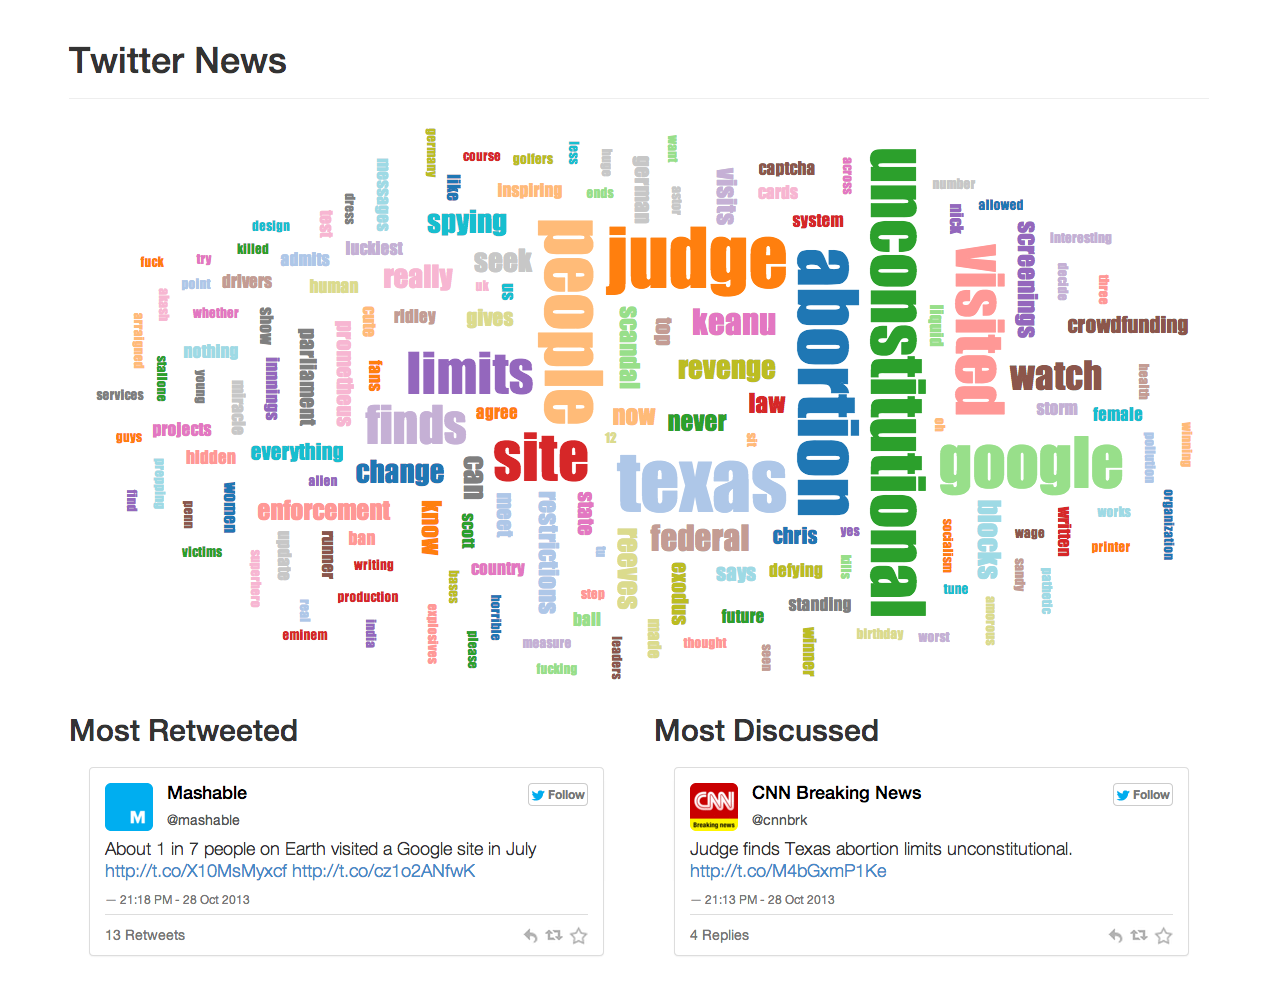
\includegraphics[width=\textwidth]{twitter_news.png}
\caption{Die TwitterNews-Anwendung}
\label{fig:die_twitternews_anwendung}
\end{figure}

% subsection die_client_seite (end)

% section umsetzung (end)

% chapter anwendung (end)